\subsubsection{Principe}

  \begin{enumerate}
    \item On initialise autant de valeurs que de nombre de classes voulues, qui correspondent aux points de gravité des classes ;
    \item Les données sont placées dans les classes en fonction de leur proximité avec l'un ou l'autre des centres de gravité ; 
    \item Ces centres sont recalculés en fonction des données affectées à la classe ; 
    \item On refait les étapes 2 et 3 jusqu'à ce que les centres de gravité n'évolue plus. 
  \end{enumerate}

\subsubsection{Implantation initiale}

  Nous avons utilisé la toolbox crée en cours de Data Mining dont la signature est : 

  \verb|function [nouveauMu, z, er]=k_moyenne(X,nbCluster,nbIteration, epsilon, initMu )|

  On utilise les valeurs de paramètres suivants : 
  \begin{itemize}
    \item X = valeur RGB des carrés ;
    \item nbCluster  = 6 ; 
    \item nbIteration = 10 (valeur de conditions d'arrêt : nombre de centres de gravité successifs à calculer) ; 
    \item epsilon = 0.01 (valeur de conditions d'arrêt : variation entre les différentes valeurs successives des centres de gravité) ; 
    \item initMu = valeur RGB des centres. 
  \end{itemize}

Les valeurs calculées sont : 
  \begin{itemize}
    \item nouveauMu = dernières valeurs des centres de gravité calculées ; 
    \item z = label des différents éléments de X ; 
    \item er = erreur concernant le nombre d'élément par classe (0 si 9 éléments par classe, 1 sinon). 
  \end{itemize}

  Cette algorithme donne des résultats précis sur des photos ayant un bon éclairage mais nous devons ajouter une condition d'arrêt dans notre algorithme de résolution qui consiste à vérifier si on a bien 9 éléments dans chaque classe. 

\subsubsection{Utilisation de la conditions : ``9 carrés par classe''}

  Afin d'adapter l'algorithme à notre application, nous avons rajouté un traitement en cas d'erreur (er=1). 

  Ainsi on modifie les labels des éléments après le K-Mean de tel façon que les classes ayant plus de 9 éléments donnent successivement un de leurs éléments aux centres ayant un déficit d'éléments, le plus proche, jusqu'à ce que ces classes atteignent chacune 9 éléments. 

  Le résultat de classification obtenu est celui de la figure~\ref{RGBnok}
  \begin{figure}[h!]
    \centering
    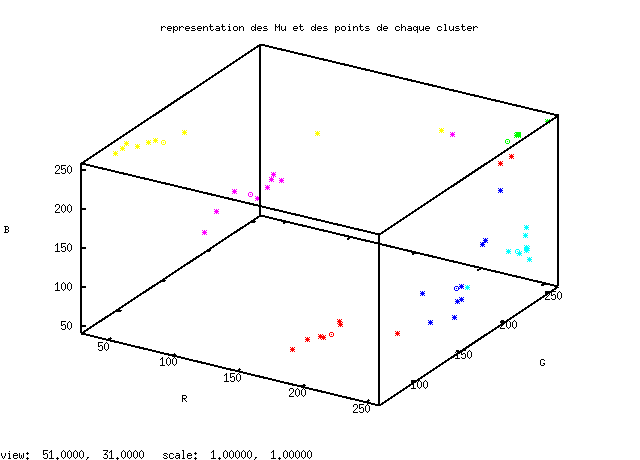
\includegraphics[width=0.5\linewidth]{./Images/RGB_nok.png}
    \caption{Représentation des données RGB des différents carrés}
    \label{RGBnok}
   \end{figure}

% \subsubsection{Limites}
% 
%   Comme il est visible sur la figure~\ref{RGBnok} sur la classe rouge notamment, les classes se retrouvent coupées en deux par d'autres classes. 
%   En effet, une classe qui a trop d'éléments peut donné un ou plusieurs de ceux-là à une classe qui est à l'opposé, si elle manque d'éléments. 
% 
% \subsubsection{Piste de résolution}
% 
%   Il faut mettre en place la condition concernant le nombre d'éléments par classe dans l'algorithme de résolution du K-Mean de tel façon que le rééquilibrage des classes se fassent entre les classes voisines. 